\documentclass[../main.tex]{subfiles}
\begin{document}
\begin{CJK*}{UTF8}{bkai}
  \subsection{多變數熱量輸送,Bessel、無因次、S-L}
  \begin{itemize}
    \item Heat transfer in a circular fin
    \begin{figure}[H]
      \centering
      \begin{tikzpicture}[>=Latex, line cap=round, line join=round, thick]
        \draw (0,-1) arc(-90:-270:0.5 and 1);
        \draw (5.5, 4) arc(90:-90:2 and 4);
        \fill[white] (0,-1) rectangle (10,1);
        \draw (4.5, -4) arc(-90:-270:2 and 4);
        \path[name path=La] (4.5, -4) arc(-90:-270:2 and 4);
        \path[name path=Ha] (0,1) -- (10,1);
        \path[name path=Hb] (0,-1) -- (10,-1);
        \path [name intersections={of=La and Ha, by=A}];
        \path [name intersections={of=La and Hb, by=B}];
        \draw (0,1) -- (A);
        \draw (0,-1) -- (B);
        \draw[dashed] (A) -- (5.5,1);
        \draw[dashed] (B) -- (5.5,-1);
        \draw (5.5,1) -- (10,1);
        \draw (5.5,-1) -- (10,-1);
        \draw (5.5,-1) arc(-90:-270:0.5 and 1);
        \draw [dashed] (5.5,1) arc(90:-90:0.5 and 1);
        \draw [dashed] (4.5,1) arc(90:-90:0.5 and 1);
        \draw [dashed] (4.5,0) ellipse (0.5 and 1);
        \draw (5.5, -4) arc(-90:-270:2 and 4);
        \draw (4.5, -4) -- (5.5, -4);
        \draw (4.5, 4) -- (5.5, 4);
        \draw (10,0) ellipse (0.5 and 1);
        \draw[dashed] (0, 1) arc(90:-90:0.5 and 1);
        \draw[dashed] (4.5, 4) arc(90:-90:2 and 4);
        \def\xShift{9}
        \def\yShift{3}
        \draw (\xShift, \yShift-0.5) rectangle (\xShift+2.25, \yShift+0.5);
        \draw (\xShift+2.75, \yShift-0.5) rectangle (\xShift+5, \yShift+0.5);
        \draw (\xShift+2.25, \yShift-2) rectangle (\xShift+2.75, \yShift+2);
        \draw[dashed] (\xShift+2.25, \yShift-0.5) -- (\xShift+2.75, \yShift-0.5);
        \draw[dashed] (\xShift+2.25, \yShift+0.5) -- (\xShift+2.75, \yShift+0.5); 
        \draw [->] (\xShift+2.5, \yShift) --(\xShift+2.5, \yShift+2.5) node[above] {$r$};
        \draw [->] (\xShift+2.5, \yShift) --(\xShift+5.5, \yShift) node[right] {$z$};
        \draw [->] (3.5, 4) -- (4.5,4);
        \draw [->] (6.5, 4) -- (5.5,4);
        \node[anchor=south] at (5,4) {$2B$};
        \node[anchor=south] at (10,1) {$T_0$};
        \node[anchor=north] at (10,5) {$T_a$, air};
        \draw [<->] (10,0) -- (10,1);
        \node[anchor=north] at (10,0) {$R_0$};
        \draw [<->] (\xShift+3,\yShift) -- (\xShift+3, \yShift+2) node[midway, right] {$R_1$};
      \end{tikzpicture}
      \caption{Circular fin}
    \end{figure}
    \begin{itemize}
      \item 假設:
      \begin{itemize}
        \item Steady state
        \item Newton's law of cooling
        \item thin-fin, heat flux at $r=R_1\approx 0$
        \item cylindrical coordinates
        \item 2D heat conduction, $T=T(r,z)$
        \item No Force Convection
      \end{itemize}
      \item Equation of Energy:
      \begin{equation}
        k\nabla^2 T = 0
      \end{equation}
      在cylindrical coordinates下:
      \begin{equation}
        \frac{1}{r}\frac{\partial}{\partial r}\left(r \frac{\partial T}{\partial r}\right) + \frac{\partial^2 T}{\partial z^2} = 0 \label{eq:circular_fin_Bessel_PDE}
      \end{equation}
      \item 邊界條件:
      \begin{align}
        & T(R_0, z) = T_0 \\
        & \frac{\partial T}{\partial r}(R_1,z) = 0\\
        & \frac{\partial T}{\partial z}(r,0) = 0,\quad\text{對稱z軸}\\
        & -k\frac{\partial T}{\partial z}(r,B) = h(T(r,B) - T_a)
      \end{align}
      \item 先假設自然對流非常的小,也就是此時在$z$方向上沒有熱傳導,為定值\\
      此時$T(r,z) = T(r)$\\
      因為對稱性,故積分$z$從0到$B$,再除以$B$,即可得到各個$r$下的平均溫度$T(r)$
      \begin{align}
        \frac{1}{B}\int_0^B \left[
          \frac{1}{r}\frac{\partial}{\partial r}\left(r \frac{\partial T}{\partial r}\right) + \frac{\partial^2 T}{\partial z^2}
        \right]  dz &= 0 \nonumber\\
        \frac{1}{r}\frac{\partial }{\partial r}\left(r\frac{\partial}{\partial r}\frac{1}{B}\int_0^B TdZ\right)
        + \frac{1}{B}\int_0^B \frac{\partial^2 T}{\partial z^2} dz &= 0 \nonumber\\
        \Rightarrow\quad \frac{1}{r}\frac{\partial}{\partial r}\left(r\frac{\partial \left<T\right>}{\partial r}\right)
        +\frac{1}{B}\frac{\partial T}{\partial z}\Big|_{z=0}^{z=B} &= 0 \nonumber\\
        \Rightarrow\quad \frac{1}{r}\frac{\partial}{\partial r}\left(r\frac{\partial \left<T\right>}{\partial r}\right)
        -\frac{h}{kB}\left(T(r,B)-T_a\right) &= 0 \nonumber\\
        \Rightarrow\quad \frac{1}{r}\frac{\partial}{\partial r}\left(r\frac{\partial T(r)}{\partial r}\right)
        -\frac{h}{kB}\left(T(r)-T_a\right) &=0 \label{eq:circular_fin_Bessel_intermediate}
      \end{align}
      於是就變ODE了\\
      P.S. 能變成1階ODE的關鍵是假設了$h$非常小,但實際上應該從邊界條件定義:
      \begin{equation}
        -k\frac{\partial T}{\partial z}(r,B) = h(T(r,B) - T_a)
      \end{equation}
      假設$\frac{\partial T}{\partial z}(r,z)=0$,代入上式
      \begin{equation}
        k\left[
          \frac{T(r,0)-T(r,B)}{B}
        \right] \approx h(T(r,B) - T_a)
      \end{equation}
      移項後得到:
      \begin{equation}
        \frac{hB}{k} \approx \frac{T(r,0)-T(r,B)}{T(r,B) - T_a}
      \end{equation}
      而這裡就出現了一個無因次群,也就是\fbox{Biot number}
      \begin{equation}
        \text{Bi} = \frac{hV/A}{k_s} = \frac{\text{內部阻力}}{\text{外部阻力}}
      \end{equation}
      因為假設了幾乎沒有$z$方向的熱傳導,所以\fbox{Biot number必須$\ll 1$}才合理\\
      關於為什麼會是阻力,可以看熱阻在卡式座標的定義(\ref{eq:thermal_resistance_flat_plate})
      以及熱對流熱阻的定義(\ref{eq:thermal_resistance_convection})
      \begin{equation}
        \text{Bi}= \frac{hL}{k_s} = \frac{L/k_s A}{1/hA} = \frac{R_k}{R_c}
      \end{equation}
      P.S. Biot Number的$k$是固體下的$k$,故會加上下標$s$\\
      容易跟Nusselt number搞混$\frac{hL}{k_f}$,這裡的$k_f$是流體的熱傳導率
      \item 解ODE(\ref{eq:circular_fin_Bessel_intermediate})式:\\
      無因次化,兩個特徵量,溫度、半徑
      \begin{equation}
        \theta = \frac{T - T_a}{T_0 - T_a},\quad r^* = \frac{r}{R_0}
      \end{equation}
      代入(\ref{eq:circular_fin_Bessel_intermediate})式,得到:
      \begin{align}
        &\frac{1}{r^\ast R_0}\frac{d}{dr^\ast}\frac{dr^\ast}{dr} \left(
          r^\ast R_0 \frac{d}{dr^\ast}\frac{d r^\ast}{dr} \left(\theta\cdot(T_0-T_a)+T_a\right)
        \right) - \frac{h}{kB}\left(
          \theta\cdot(T_0-T_a)+T_a - T_a
        \right) \nonumber\\
        \Rightarrow\quad & \frac{1}{r^\ast R_0}\frac{d}{dr^\ast}\frac{1}{R_0} \left(
          r^\ast R_0 \frac{d}{dr^\ast}\frac{1}{R_0} \left(\theta\cdot(T_0-T_a)+T_a\right)
        \right) - \frac{h}{kB}\theta(T_0-T_a) \nonumber\\
        \Rightarrow\quad & \frac{T_0 - T_a}{R_0^2} \left[
          \frac{1}{r^\ast}\frac{d}{dr^\ast}\left(
            r^\ast \frac{d\theta}{dr^\ast}
          \right)
        \right] - \frac{h}{kB}\theta(T_0-T_a)  = 0 \nonumber\\
        \Rightarrow\quad & \frac{1}{r^\ast}\frac{d}{dr^\ast}\left(
          r^\ast \frac{d\theta}{dr^\ast}
        \right) - \frac{h R_0^2}{kB}\theta = 0 \nonumber\\
        \Rightarrow\quad & \frac{1}{r^\ast}\left(
          \frac{d\theta}{dr^\ast} + r^\ast \frac{d^2\theta}{d{r^\ast}^2}
        \right) - \frac{h R_0^2}{kB}\theta = 0 \nonumber\\
        \Rightarrow\quad & r^\ast \frac{d^2\theta}{d{r^\ast}^2} + \frac{d\theta}{dr^\ast}
        - \frac{h R_0^2}{kB} r^\ast \theta = 0 \quad 
        \text{乘上}r^\ast\text{變成Bessel} \nonumber\\
        \Rightarrow\quad & {r^\ast}^2 \frac{d^2\theta}{d{r^\ast}^2} + r^\ast \frac{d\theta}{dr^\ast}
        - \frac{h R_0^2}{kB} {r^\ast}^2 \theta = 0 \label{eq:circular_fin_Bessel_equation}
      \end{align}
      \item 此時Bondary Conditions變成:
      \begin{align}
        & \theta(1) = 1 \\
        & \frac{d\theta}{dr^\ast}(R_1^\ast) = 0,\quad R_1^\ast = \frac{R_1}{R_0}
      \end{align}
      \item 我們有General Bessel Equation:
      \begin{equation}
        x^2 \frac{d^2y}{dx^2}+x(a+2bx^r)\frac{dy}{dx} + \left[
          c+dx^{2s}-b(1-a-r)x^r + b^2 x^{2r}
        \right]y = 0
      \end{equation}
      其解為:
      \begin{equation}
        y(x)=x^{\frac{1-a}{2}} e^{- \frac{b x^r}{r}} Z_p\left(
          \frac{\sqrt{d}}{s}x^s\right),\quad P = \frac{1}{s}\sqrt{\frac{(1-a)^2}{2} -c}
      \end{equation}
      如果$\frac{d}{s}$是實數,則解為$J_P,Y_P$\\
      如果$\frac{d}{s}$是虛數,則解為$I_P,K_P$
      \item 比較係數後發現:
      \begin{equation}
        a=1,~b=0,~r=1,~s=1,~d=-\frac{h R_0^2}{kB},~c=0
      \end{equation}
      而
      \begin{equation}
        P = \frac{1}{1}\sqrt{\frac{(1-1)^2}{2}-0} = 0
      \end{equation}
      且
      \begin{equation}
        \frac{d}{s} = -\frac{h R_0^2}{kB} < 0
      \end{equation}
      故解為$I_0,K_0$,因此(\ref{eq:circular_fin_Bessel_equation})式的General Solution為:
      \begin{equation}
        \theta(r^\ast) = C_1 I_0\left(\sqrt{\frac{h R_0^2}{kB}} r^\ast\right)
        + C_2 K_0\left(\sqrt{\frac{h R_0^2}{kB}} r^\ast\right)
      \end{equation}
      \item 代入邊界條件,解得:
      \begin{align}
        & 1 = C_1 I_0\left(\sqrt{\frac{h R_0^2}{kB}}\right)
        + C_2 K_0\left(\sqrt{\frac{h R_0^2}{kB}}\right) \label{eq:circular_fin_Bessel_BC1}\\
        & 0 = C_1 \sqrt{\frac{h R_0^2}{kB}} I_1\left(\sqrt{\frac{h R_0^2}{kB}} R_1^\ast\right)
        - C_2 \sqrt{\frac{h R_0^2}{kB}} K_1\left(\sqrt{\frac{h R_0^2}{kB}} R_1^\ast\right) \label{eq:circular_fin_Bessel_BC2}
      \end{align}
      由Bessel函數的性質:
      \begin{equation}
        \frac{d}{dx}I_0(\alpha x) = \alpha I_1(\alpha x),\quad
        \frac{d}{dx}K_0(\alpha x) = -\alpha K_1(\alpha x)
      \end{equation}
      令
      \begin{equation}
        \alpha = \sqrt{\frac{h R_0^2}{kB}}
      \end{equation}
      \item (\ref{eq:circular_fin_Bessel_BC2})式可改寫為
      \begin{equation}
        0 = C_1\alpha I_1\left(\alpha R_1^\ast\right)
        - C_2 \alpha K_1\left(\alpha R_1^\ast\right) \label{eq:circular_fin_Bessel_BC2_modified}
      \end{equation}
      \item 將(\ref{eq:circular_fin_Bessel_BC1})乘上$K_1\left(\alpha R_1^\ast\right)$
      加上(\ref{eq:circular_fin_Bessel_BC2_modified})乘上$K_0\left(\alpha \right)$\\
      削去$C_2$得到:
      \begin{align}
        & \alpha  K_1\left(\alpha  R_1^\ast\right)
        = C_1 \left[
          \alpha K_1\left(\alpha  R_1^\ast\right) I_0\left(\alpha \right)
          + \alpha K_0\left(\alpha \right) I_1\left(\alpha  R_1^\ast\right)
        \right] \nonumber\\
        \Rightarrow\quad & C_1 = \frac{K_1\left(\alpha  R_1^\ast\right)}
        {K_1\left(\alpha  R_1^\ast\right) I_0\left(\alpha \right)
          + K_0\left(\alpha \right) I_1\left(\alpha  R_1^\ast\right)} \label{eq:circular_fin_Bessel_C1}
      \end{align}
      \item 將(\ref{eq:circular_fin_Bessel_BC1})乘上$\alpha I_1\left(\alpha  R_1^\ast\right)$
      減去(\ref{eq:circular_fin_Bessel_BC2_modified})乘上$I_0\left(\alpha \right)$\\
      削去$C_1$得到:
      \begin{align}
        & \alpha  I_1\left(\alpha  R_1^\ast\right)
        = C_2 \left[
          \alpha K_0\left(\alpha \right) I_1\left(\alpha  R_1^\ast\right)
          + \alpha I_0\left(\alpha \right) K_1\left(\alpha  R_1^\ast\right)
        \right] \nonumber\\
        \Rightarrow\quad & C_2 = \frac{I_1\left(\alpha  R_1^\ast\right)}
        {K_0\left(\alpha \right) I_1\left(\alpha  R_1^\ast\right)
          + I_0\left(\alpha \right) K_1\left(\alpha  R_1^\ast\right)} \label{eq:circular_fin_Bessel_C2}
      \end{align}
      \item 最後代入(\ref{eq:circular_fin_Bessel_C1})、(\ref{eq:circular_fin_Bessel_C2})回General Solution,得到最終解:
      \begin{align}
        \theta(r^\ast) &= \frac{K_1\left(\alpha  R_1^\ast\right) I_0\left(\alpha r^\ast\right)
        + I_1\left(\alpha  R_1^\ast\right) K_0\left(\alpha r^\ast\right)}{
          K_1\left(\alpha  R_1^\ast\right) I_0\left(\alpha \right)
          + K_0\left(\alpha \right) I_1\left(\alpha  R_1^\ast\right)
        } \nonumber\\
      &= \frac{K_0\left(\alpha r^\ast \right)
       + \frac{K_1\left(\alpha R_1^\ast \right)}{I_1\left(\alpha R_1^\ast \right)} I_0\left(\alpha r^\ast \right)}{
        K_0\left(\alpha \right) 
        + \frac{K_1\left(\alpha R_1^\ast \right)}{I_1\left(\alpha R_1^\ast \right)} I_0\left(\alpha \right)
      } \label{eq:circular_fin_Bessel_final_solution}
      \end{align}
      \item 計算熱效率值$\eta_f$:
      \begin{align}
        \eta_f &= \frac{\text{實際散熱量}}{\text{最大可能散熱量}}\nonumber\\
        &= \frac{\left(2\pi R_0\cdot 2B\right)\left(-k\frac{\partial T}{\partial r}\big|_{r=R_0}\right)}
        {2\pi\left(R_1^2-R_0^2\right)h_f(T_0 - T_a)} \nonumber\\
        &= \frac{2k BR_0}{h_f\left(R_1^2 - R_0^2\right)\left(T_0-T_a\right)} \left(-\frac{\partial T}{\partial r}\bigg|_{r=R_0}\right) 
        \label{eq:circular_fin_efficiency}
      \end{align}
      而其中$-\frac{\partial T}{\partial r}\big|_{r=R_0}$可由(\ref{eq:circular_fin_Bessel_final_solution})式求出
      \begin{align}
        -\frac{\partial T}{\partial r}\bigg|_{r=R_0} &=
        -\frac{T_0 - T_a}{R_0} \frac{d\theta}{dr^\ast}\bigg|_{r^\ast=1} \nonumber\\
        & = -\frac{T_0 - T_a}{R_0} \left[\frac{
          -\alpha\left( K_1(\alpha) - \frac{K_1(\alpha R_1^\ast)}{I_1(\alpha R_1^\ast)}I_1(\alpha)\right)
        }{
          K_0(\alpha) + \frac{K_1(\alpha R_1^\ast)}{I_1(\alpha R_1^\ast)} I_0(\alpha)
        } \right]
      \end{align}
      代回(\ref{eq:circular_fin_efficiency})式,即可求出熱效率值
      \begin{align}
        \eta_f & = \frac{2 k BR_0}{h_f\left(R_1^2 - R_0^2\right)\left(T_0-T_a\right)} \cdot \frac{T_0 - T_a}{R_0}
        \left[\frac{
          \alpha\left( K_1(\alpha) - \frac{K_1(\alpha R_1^\ast)}{I_1(\alpha R_1^\ast)}I_1(\alpha)\right)
        }{
          K_0(\alpha) + \frac{K_1(\alpha R_1^\ast)}{I_1(\alpha R_1^\ast)} I_0(\alpha)
        } \right] \nonumber\\
        & = \frac{2 k B \alpha}{h_f\left(R_1^2 - R_0^2\right)}
        \left[\frac{
          K_1(\alpha) - \frac{K_1(\alpha R_1^\ast)}{I_1(\alpha R_1^\ast)}I_1(\alpha)
        }{
          K_0(\alpha) + \frac{K_1(\alpha R_1^\ast)}{I_1(\alpha R_1^\ast)} I_0(\alpha)
        } \right]
      \end{align}
      我們令整個中刮號內為$F(\alpha, R_1^\ast)$\\
      且$\alpha^2 = \frac{h R_0^2}{kB}= \text{Bi}\frac{R_0^2}{B^2}$\\
      $\alpha = \sqrt{\text{Bi}}\frac{R_0}{B}$\\
      最終熱效率值為:
      \begin{align}
        \eta_f &= \frac{2 k B \alpha}{h_f\left(R_1^2 - R_0^2\right)} F(\alpha, R_1^\ast) \nonumber\\
        &= \frac{2 k B \sqrt{\text{Bi}}\frac{R_0}{B}}{h_f\left(R_1^2 - R_0^2\right)} F(\alpha, R_1^\ast) \nonumber\\
        &= \frac{2 {\color{red}k} B \cancel{R_0} \sqrt{\text{Bi}}}{{\color{red}h_f B} R_0^{\cancel{2}}\left(R_1^{2\ast}-1\right)} F(\alpha, R_1^\ast) \nonumber\\
        &= \frac{2 B \sqrt{\text{Bi}}}{R_0\left(R_1^{2\ast}-1\right)\text{Bi}} F(\alpha, R_1^\ast) \nonumber\\
        &= \frac{2B}{R_0\left(R_1^{2\ast}-1\right)\sqrt{\text{Bi}}} F(\alpha, R_1^\ast) \label{eq:circular_fin_efficiency_final}
      \end{align}
      \item 那2維的話呢,回到最原本的PDE(\ref{eq:circular_fin_Bessel_PDE})式
      \begin{equation}
        \frac{1}{r}\frac{\partial}{\partial r}\left(r \frac{\partial T}{\partial r}\right) + \frac{\partial^2 T}{\partial z^2} = 0
      \end{equation}
      我們對$z$方向的特徵長度為$B$,故再加上一無因次變數$z^\ast = \frac{z}{B}$,則PDE變成:
      \begin{align}
        &\frac{1}{r^\ast R_0}\frac{\partial}{\partial r^\ast}\frac{dr^\ast}{dr} \left(
          r^\ast R_0 \frac{\partial}{\partial r^\ast}\frac{d r^\ast}{dr} T
        \right) + \frac{\partial^2}{\partial z^{\ast 2}}\frac{d z^\ast}{dz}\frac{d z^\ast}{dz} T = 0 \nonumber\\
        \Rightarrow\quad & \frac{1}{r^\ast R_0}\frac{\partial}{\partial r^\ast}\frac{1}{R_0} \left(
          r^\ast R_0 \frac{\partial}{\partial r^\ast}\frac{1}{R_0} T
        \right) + \frac{\partial^2}{\partial z^{\ast 2}}\frac{1}{B^2} T = 0 \nonumber\\
        \Rightarrow\quad & \frac{1}{r^\ast}\frac{\partial}{\partial r^\ast}\left(
          r^\ast \frac{\partial T}{\partial r^\ast}
        \right) + \frac{R_0^2}{B^2} \frac{\partial^2 T}{\partial z^{\ast 2}} = 0 \label{eq:circular_fin_Bessel_2D_PDE}
      \end{align}
      於是我們令$\beta= \frac{B}{R_0}$,則(\ref{eq:circular_fin_Bessel_2D_PDE})式變成:
      \begin{equation}
        \frac{1}{r^\ast}\frac{\partial}{\partial r^\ast}\left(
          r^\ast \frac{\partial T}{\partial r^\ast}
        \right) + \frac{1}{\beta^2} \frac{\partial^2 T}{\partial z^{\ast 2}} = 0
      \end{equation}
      \item 此時邊界條件變成:
      \begin{align}
         \theta(1, z^\ast) &= 1 \\
         \frac{\partial \theta}{\partial r^\ast}(R_1^\ast,z^\ast) &= 0,\quad R_1^\ast = \frac{R_1}{R_0}\\
         \frac{\partial \theta}{\partial z^\ast}(r^\ast,0) &= 0,\quad\text{對稱z軸}\\
         -\frac{\partial \theta}{\partial z^\ast}(r^\ast, 1)& = -\text{Bi} \cdot \theta(r^\ast, 1)
      \end{align}
      \item 可用分離變數法求解,令:
      \begin{equation}
        \theta(r^\ast, z^\ast) = R(r^\ast) Z(z^\ast)
      \end{equation}
      代入PDE,得到:
      \begin{align}
        & \frac{1}{r^\ast}\frac{d}{dr^\ast}\left(
          r^\ast \frac{dR}{dr^\ast} Z
        \right) + \frac{1}{\beta^2} R \frac{d^2 Z}{d z^{\ast 2}} = 0 \nonumber\\
        \Rightarrow\quad & \frac{Z}{r^\ast}\frac{d}{dr^\ast}\left(
          r^\ast \frac{dR}{dr^\ast}
        \right) + \frac{R}{\beta^2} \frac{d^2 Z}{d z^{\ast 2}} = 0 \nonumber\\
        \Rightarrow\quad & \frac{1}{R}\frac{1}{r^\ast}\frac{d}{dr^\ast}\left(
          r^\ast \frac{dR}{dr^\ast}
        \right) + \frac{1}{Z}\frac{1}{\beta^2} \frac{d^2 Z}{d z^{\ast 2}} = 0 \nonumber\\
        \Rightarrow\quad & \frac{1}{R}\frac{1}{r^\ast}\frac{d}{dr^\ast}\left(
          r^\ast \frac{dR}{dr^\ast}
        \right) = - \frac{1}{Z}\frac{1}{\beta^2} \frac{d^2 Z}{d z^{\ast 2}} = -\lambda^2
      \end{align}
      \item 選正的Homogeneous Boundary Conditions,再用S-L解決:
      \begin{equation}
        Z'' + \lambda^2 \beta^2 Z = 0 \implies Z(z^\ast) = C_1 \sin(\beta \lambda z^\ast) + C_2 \cos(\beta \lambda z^\ast)
      \end{equation}
      至於另外一邊,就會跟之前一樣,得到Bessel方程式:
      \begin{equation}
        r^{\ast 2} R'' + r^\ast R' + \left(-\lambda^2 r^{\ast 2}\right) R = 0 \implies
        R(r^\ast) = C_3 I_0(\lambda r^\ast) + C_4 K_0(\lambda r^\ast)
      \end{equation}
      \item 最終解為:
      \begin{equation}
        \theta(r^\ast, z^\ast) = \left[
          C_3 I_0(\lambda r^\ast) + C_4 K_0(\lambda r^\ast)
        \right] \left[
          C_1 \sin(\beta \lambda z^\ast) + C_2 \cos(\beta \lambda z^\ast)
        \right]
      \end{equation}
      \item 接下來就代入邊界條件求解$\lambda$與各個常數\\
      當代入$\theta(1, z^\ast)=1$時,會發現全部都是0,所以是個S-L問題\\
      我們先解其他的,再用正交條件來把這個邊界條件解出無窮級數的各項係數
      \item $\frac{\partial \theta}{\partial r^\ast}(R_1^\ast,z^\ast) = 0$
      \begin{align}
        \frac{\partial \theta}{\partial r^\ast} &= \left[
          C_3 \lambda I_0'(\lambda r^\ast) + C_4 \lambda K_0'(\lambda r^\ast)
        \right] \left[
          C_1 \sin(\beta \lambda z^\ast) + C_2 \cos(\beta \lambda z^\ast)
        \right] \nonumber\\
        &=\left[
          C_3 \lambda I_1(\lambda r^\ast) - C_4 \lambda K_1(\lambda r^\ast)
        \right] \left[
          C_1 \sin(\beta \lambda z^\ast) + C_2 \cos(\beta \lambda z^\ast)
        \right]
      \end{align}
      代入邊界條件,得到:
      \begin{equation}
        \left[
          C_3 \lambda I_1(\lambda R_1^\ast) - C_4 \lambda K_1(\lambda R_1^\ast)
        \right] \left[
          C_1 \sin(\beta \lambda z^\ast) + C_2 \cos(\beta \lambda z^\ast)
        \right] = 0
      \end{equation}
      因為要對所有$z^\ast$成立,故:
      \begin{equation}
        C_3 \lambda I_1(\lambda R_1^\ast) - C_4 \lambda K_1(\lambda R_1^\ast) = 0
      \end{equation}
      解得:
      \begin{equation}
        C_3 = \frac{C_4 K_1(\lambda R_1^\ast)}{I_1(\lambda R_1^\ast)}
      \end{equation}
      代回$R(r^\ast)$,可減併為:
      \begin{equation}
        R(r^\ast) = C_4 \left[
          \frac{K_1(\lambda R_1^\ast)}{I_1(\lambda R_1^\ast)} I_0(\lambda r^\ast) + K_0(\lambda r^\ast)
        \right]
      \end{equation}
      \item $\frac{\partial \theta}{\partial z^\ast}(r^\ast,0) = 0$
      \begin{align}
        \frac{\partial \theta}{\partial z^\ast} &= \left[
          C_3 I_0(\lambda r^\ast) + C_4 K_0(\lambda r^\ast)
        \right] \left[
          C_1 \beta \lambda \cos(\beta \lambda z^\ast) - C_2 \beta \lambda \sin(\beta \lambda z^\ast)
        \right] \nonumber\\
        & = \beta \lambda \left[
          C_3 I_0(\lambda r^\ast) + C_4 K_0(\lambda r^\ast)
        \right] \left[
          C_1 \cos(\beta \lambda z^\ast) - C_2 \sin(\beta \lambda z^\ast)
        \right]
      \end{align}
      代入邊界條件,得到:
      \begin{equation}
        \beta \lambda \left[
          C_3 I_0(\lambda r^\ast) + C_4 K_0(\lambda r^\ast)
        \right] C_1 = 0
      \end{equation}
      故$C_1=0$\\
      代回$Z(z^\ast)$,可減併為:
      \begin{equation}
        Z(z^\ast) = C_2 \cos(\beta \lambda z^\ast)
      \end{equation}
      而$\theta(r^\ast, z^\ast)$可以進一步合併$C_2 C_4 = C_5$,得到:
      \begin{equation}
        \theta(r^\ast, z^\ast) = C_5 \left[
          \frac{K_1(\lambda R_1^\ast)}{I_1(\lambda R_1^\ast)} I_0(\lambda r^\ast) + K_0(\lambda r^\ast)
        \right] \cos(\beta \lambda z^\ast)
      \end{equation}
      \item 代入第四個邊界條件,$-\frac{\partial \theta}{\partial z^\ast}(r^\ast, 1) = -\text{Bi} \cdot \theta(r^\ast, 1)$
      \begin{align}
        & -C_5 \beta \lambda\sin(\beta \lambda)\left[
          \frac{K_1(\lambda R_1^\ast)}{I_1(\lambda R_1^\ast)} I_0(\lambda r^\ast) + K_0(\lambda r^\ast)
        \right] \nonumber\\
        &\quad\quad + \text{Bi} \cdot C_5 \cos(\beta \lambda)\left[
          \frac{K_1(\lambda R_1^\ast)}{I_1(\lambda R_1^\ast)} I_0(\lambda r^\ast) + K_0(\lambda r^\ast)
        \right] =0 \nonumber\\
        \Rightarrow\quad & C_5 \left[
          \frac{K_1(\lambda R_1^\ast)}{I_1(\lambda R_1^\ast)} I_0(\lambda r^\ast) + K_0(\lambda r^\ast)
        \right] \left(-\beta \lambda\sin(\beta \lambda) + \text{Bi} \cdot \cos(\beta \lambda)\right) = 0
      \end{align}
      因為要對所有$r^\ast$成立,故:
      \begin{equation}
        -\beta \lambda\sin(\beta \lambda) + \text{Bi} \cdot \cos(\beta \lambda) = 0
      \end{equation}
      \item 故特徵值$\lambda_n$需滿足:
      \begin{equation}
        \cot(\beta \lambda_n) = \frac{\beta\lambda_n}{\text{Bi}}
      \end{equation}
      這些就是在下圖中與紅線交點的那些值(紅線斜率為$\frac{1}{\text{Bi}}$)
      \begin{figure}[H]
        \centering
        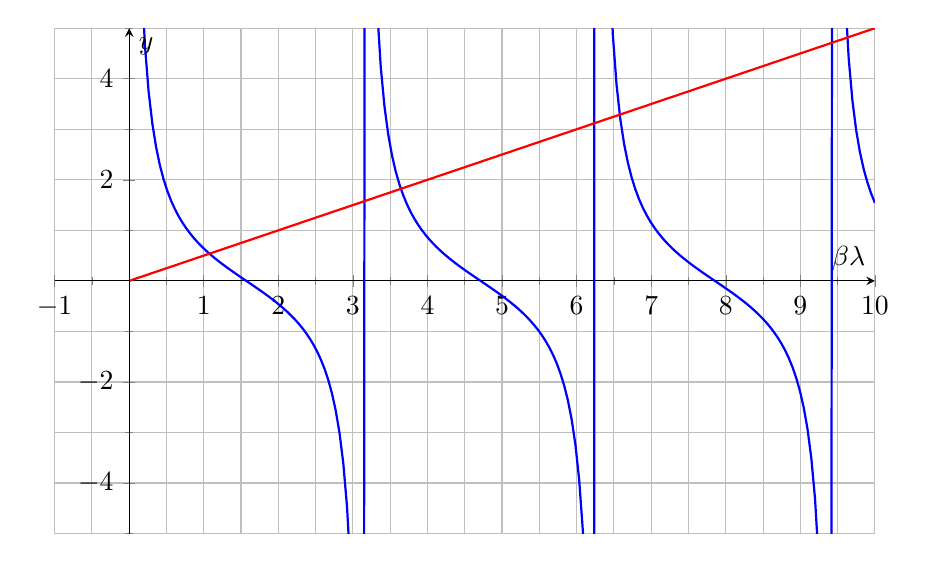
\begin{tikzpicture}
          \begin{axis}[
            axis lines = middle,
            xlabel = {$\beta \lambda$},
            ylabel = {$y$},
            ymin = -5, ymax = 5,
            xmin = -1, xmax = 10,
            domain=0.01:10,
            samples=200,
            width=12cm,
            height=8cm,
            grid=both,
            minor tick num=1,
            ]
            \addplot[blue, thick] {cot(deg(x))};
            \addplot[red, thick] {x/2}; % 假設 Bi = 2
          \end{axis}
        \end{tikzpicture}
        \caption{cot 特徵值的圖解法示意圖}
      \end{figure}
      總之,我們還是確實的知道了每個$\lambda_n$的值,只是無法用代數表示他\\
      而所有的解,就是所有$\lambda_n$的線性組合:
      \begin{equation}
        \theta(r^\ast, z^\ast) = \sum_{n=1}^\infty C_n \left[
          \frac{K_1(\lambda_n R_1^\ast)}{I_1(\lambda_n R_1^\ast)} I_0(\lambda_n r^\ast) + K_0(\lambda_n r^\ast)
        \right] \cos(\beta \lambda_n z^\ast)
      \end{equation}
      而每一項的係數$C_n$,就要用到最後一個邊界條件$\theta(1, z^\ast) = 1$來求解
      \begin{equation}
        1 = \sum_{n=1}^\infty C_n \left[
          \frac{K_1(\lambda_n R_1^\ast)}{I_1(\lambda_n R_1^\ast)} I_0(\lambda_n) + K_0(\lambda_n)
        \right]\cos(\beta \lambda_n z^\ast)
      \end{equation}
      \item 利用正交條件\\
      假設中刮號內的函數為$A_n$是已知的,只是太長了
      \begin{equation}
        1 = \sum_{n=1}^\infty C_n A_n \cos(\beta \lambda_n z^\ast)
      \end{equation}
      兩邊乘上$\cos(\beta \lambda_m z^\ast)$並對$z^\ast$從0到1積分
      \begin{align}
        & \int_0^1 1 \cdot \cos(\beta \lambda_m z^\ast) dz^\ast
        = \int_0^1 \sum_{n=1}^\infty C_n A_n \cos(\beta \lambda_n z^\ast) \cos(\beta \lambda_m z^\ast) dz^\ast \nonumber\\
        \Rightarrow\quad & \int_0^1 \cos(\beta \lambda_m z^\ast) dz^\ast
        = \sum_{n=1}^\infty C_n A_n \int_0^1 \cos(\beta \lambda_n z^\ast) \cos(\beta \lambda_m z^\ast) dz^\ast \nonumber
      \end{align}
      \item 利用正交條件:
      \begin{align}
        \Rightarrow\quad & \frac{\sin(\beta \lambda_m)}{\beta \lambda_m}
        = C_m A_m \int_0^1 \cos^2(\beta \lambda_m z^\ast) dz^\ast \nonumber\\
        \Rightarrow\quad & \frac{\sin(\beta \lambda_m)}{\beta \lambda_m}
        = C_m A_m \left[
          \frac{z^\ast}{2} + \frac{\sin(2\beta \lambda_m z^\ast)}{4\beta \lambda_m}
        \right]_0^1 \nonumber\\
        \Rightarrow\quad & \frac{\sin(\beta \lambda_m)}{\beta \lambda_m}
        = C_m A_m \left(
          \frac{1}{2} + \frac{\sin(2\beta \lambda_m)}{4\beta \lambda_m}
        \right) \nonumber\\
        \Rightarrow\quad & C_m = \frac{\sin(\beta \lambda_m)}{\beta \lambda_m A_m \left(
          \frac{1}{2} + \frac{\sin(2\beta \lambda_m)}{4\beta \lambda_m}
        \right)} \label{eq:circular_fin_Bessel_2D_Cm}
      \end{align}
      \item 最終2D解為:
      \begin{equation}
        \theta(r^\ast, z^\ast) = \sum_{n=1}^\infty \frac{\sin(\beta \lambda_n)}{\beta \lambda_n A_n \left(
          \frac{1}{2} + \frac{\sin(2\beta \lambda_n)}{4\beta \lambda_n}
        \right)}\left[
          \frac{K_1(\lambda_n R_1^\ast)}{I_1(\lambda_n R_1^\ast)} I_0(\lambda_n r^\ast) + K_0(\lambda_n r^\ast)
        \right] \cos(\beta \lambda_n z^\ast)
      \end{equation}
      其中$A_n$為:
      \begin{equation}
        \frac{K_1(\lambda_n R_1^\ast)}{I_1(\lambda_n R_1^\ast)} I_0(\lambda_n) + K_0(\lambda_n)
      \end{equation}
    \end{itemize}
  \end{itemize}
\end{CJK*}
\end{document}